\documentclass{article}
\usepackage{graphicx}
\usepackage{amsmath}
\usepackage{booktabs}
\usepackage{siunitx}
\usepackage{float}

\title{Assignment 4 - EE4725 Quasi Optical Systems}
\author{Daniel Tyukov \\ Student Number: 5714699 \\ Microelectronics, TU Delft}
\date{March 2026}

\begin{document}

\maketitle

\tableofcontents
\newpage

%% ====================================================================
\section{System Parameters}
%% ====================================================================

The system under analysis is a parabolic reflector antenna with a circular aperture feed, analyzed in reception using Fourier Optics (FO). The geometry is shown in Fig.~1 of the assignment: the reflector opens toward the feed, which sits at the focal plane with its current directed along $\hat{x}$.

\begin{itemize}
\item Operating frequency: $f = \SI{220}{GHz}$, wavelength $\lambda_0 = c/f = \SI{1.3636}{mm}$, wavenumber $k_0 = 2\pi/\lambda_0$
\item Free-space impedance: $\zeta_0 = 120\pi\;\Omega$
\item Feed: circular aperture with linearly \textbf{x-polarized} uniform amplitude current distribution, diameter $D_f = 3.6\lambda_0 = \SI{4.909}{mm}$, radius $a = D_f/2 = 1.8\lambda_0$
\item Parabolic reflector: diameter $D_r = 130\lambda_0 = \SI{177.3}{mm}$, f-number $f_\# = 1.8$, focal length $F = f_\# D_r = \SI{319.1}{mm}$
\item Reflector half-angle: $\theta_0 = 2\arctan\!\left(\dfrac{D_r}{4F}\right) = 15.81^\circ$
\item Incident plane wave: x-polarized, amplitude $E_0^{PW} = \SI{1}{V/m}$
\end{itemize}

The FO sphere is centered at the focal point with radius $R = F$. The analysis uses the spectral Green's function (SGF) for the feed far field, and the Geometrical Optics (GO) field for the reflected plane wave on the FO sphere.

%% ====================================================================
\section{Part 1: Feed at the Center of the Focal Plane}
%% ====================================================================

%% -------------------------------------------
\subsection{Q1.1 -- Q1.2: GO Field and Feed Far Field on the FO Sphere}
%% -------------------------------------------

\subsubsection{GO field (Q1.1)}

For an x-polarized broadside plane wave ($\theta_i = 0^\circ$, $\phi_i = 0^\circ$) incident on the parabolic reflector, the GO electric field on the equivalent FO sphere of radius $R = F$ is:
\begin{equation}\label{eq:GO_field}
\vec{e}_r^{\,GO}(\theta,\phi) = -\frac{2}{1+\cos\theta}\left(\cos\phi\,\hat{\theta} - \sin\phi\,\hat{\phi}\right) E_0^{PW}
\end{equation}

The factor $S(\theta) = 2/(1+\cos\theta)$ is the parabolic spreading factor. It accounts for the reflector geometry concentrating energy more at larger $\theta$ (edges) than at the center. For $f_\# = 1.8$, the spreading factor varies from $S(0) = 1.0$ to $S(\theta_0) = 1.04$---a mere 4\% variation across the FO sphere. This near-uniformity is characteristic of high $f_\#$ reflectors.

\subsubsection{Feed far field (Q1.2)}

The feed far field is computed via the free-space spectral Green's function. For an x-polarized uniform circular current distribution:
\begin{equation}\label{eq:feed_ff}
\vec{E}^{a}_{far}(\theta,\phi) = \frac{jk_z}{2\pi r}\,e^{-jk_0 r}\;\bar{\bar{G}}^{ej}_{xx}(k_x,k_y)\;\widetilde{J}_x(k_\perp)
\end{equation}
where $\widetilde{J}_x(k_\perp) = \pi a^2 \cdot 2J_1(k_\perp a)/(k_\perp a)$ is the Fourier transform of the uniform circular aperture, and the x-column of the SGF $(G_{xx}, G_{yx}, G_{zx})$ is used instead of the y-column from Assignment~2.

The first null of the Airy pattern occurs at $\theta_{\text{null}} = \arcsin(1.22\lambda_0/D_f) = 19.8^\circ$, which is beyond the reflector edge at $\theta_0 = 15.81^\circ$.

\begin{figure}[H]
\centering
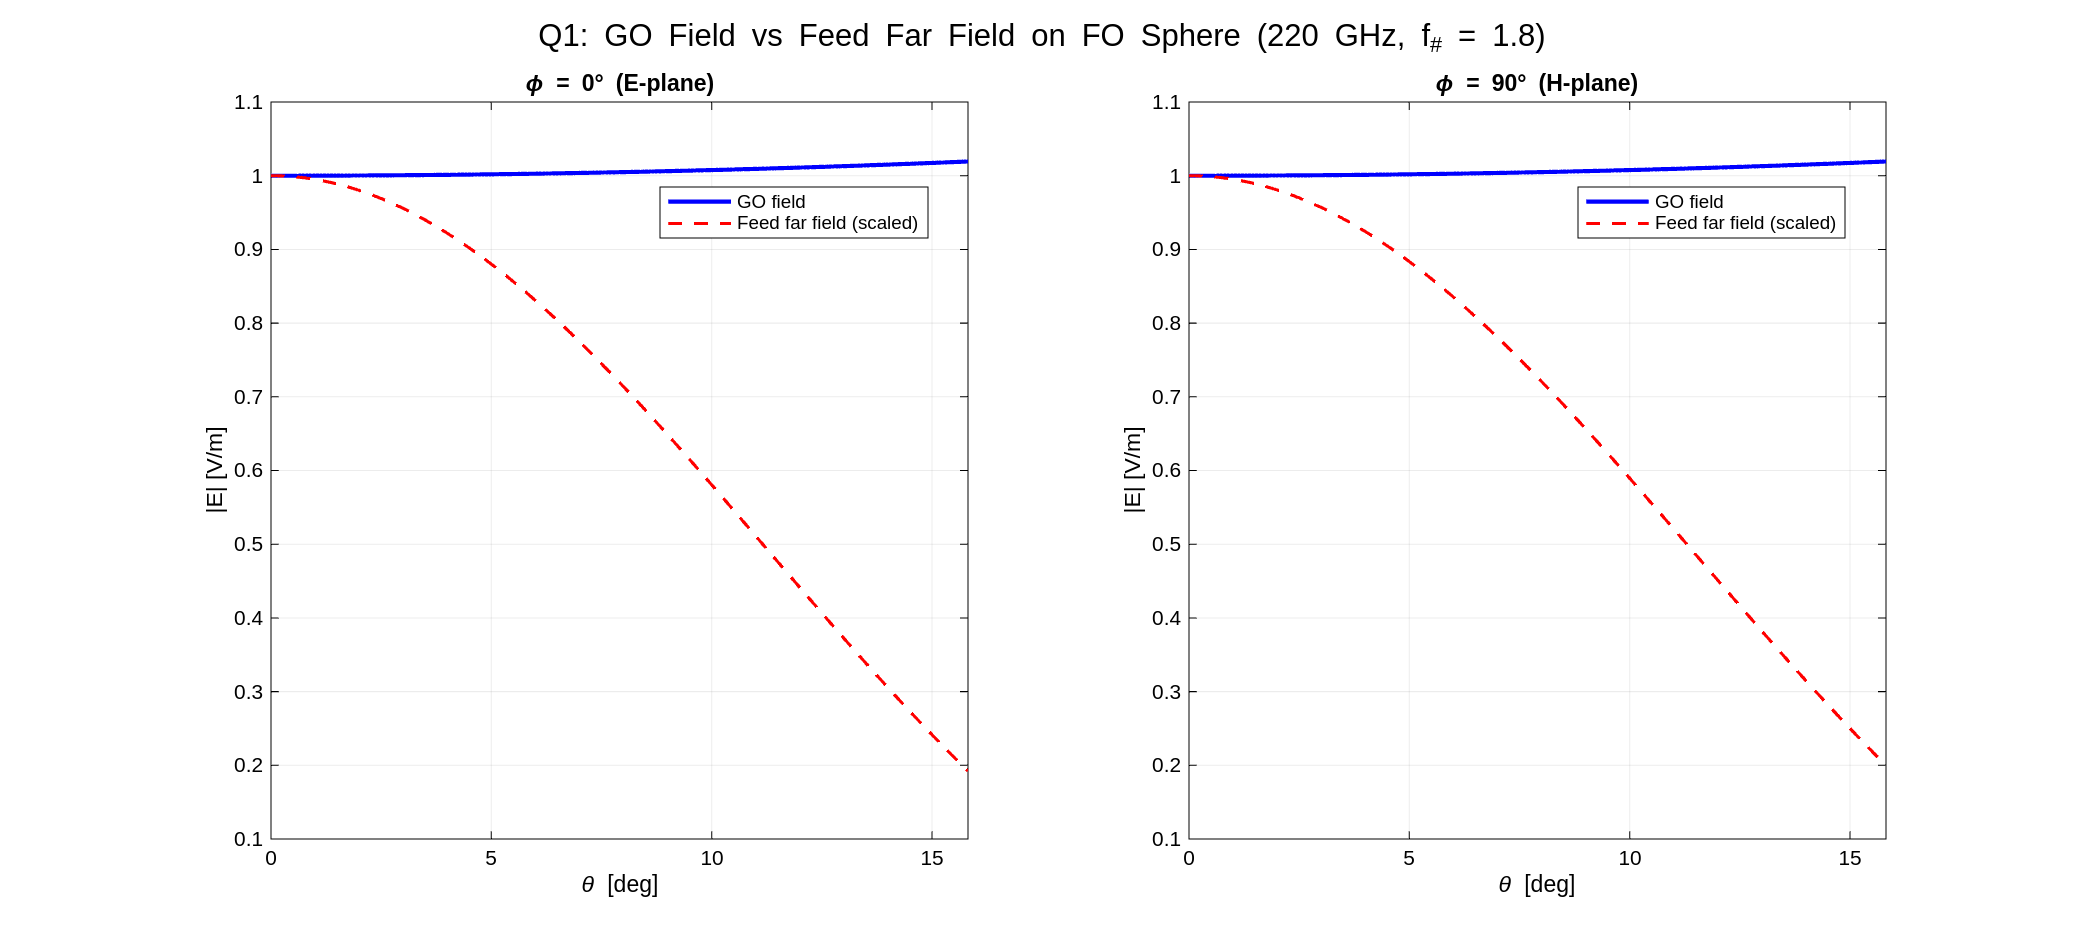
\includegraphics[width=0.95\textwidth]{figures/Q1_GO_and_feed.png}
\caption{GO field (blue) and scaled feed far field (red dashed) on the FO sphere in the $\phi = 0^\circ$ (E-plane) and $\phi = 90^\circ$ (H-plane) planes.}
\label{fig:q1_linear}
\end{figure}

\begin{figure}[H]
\centering
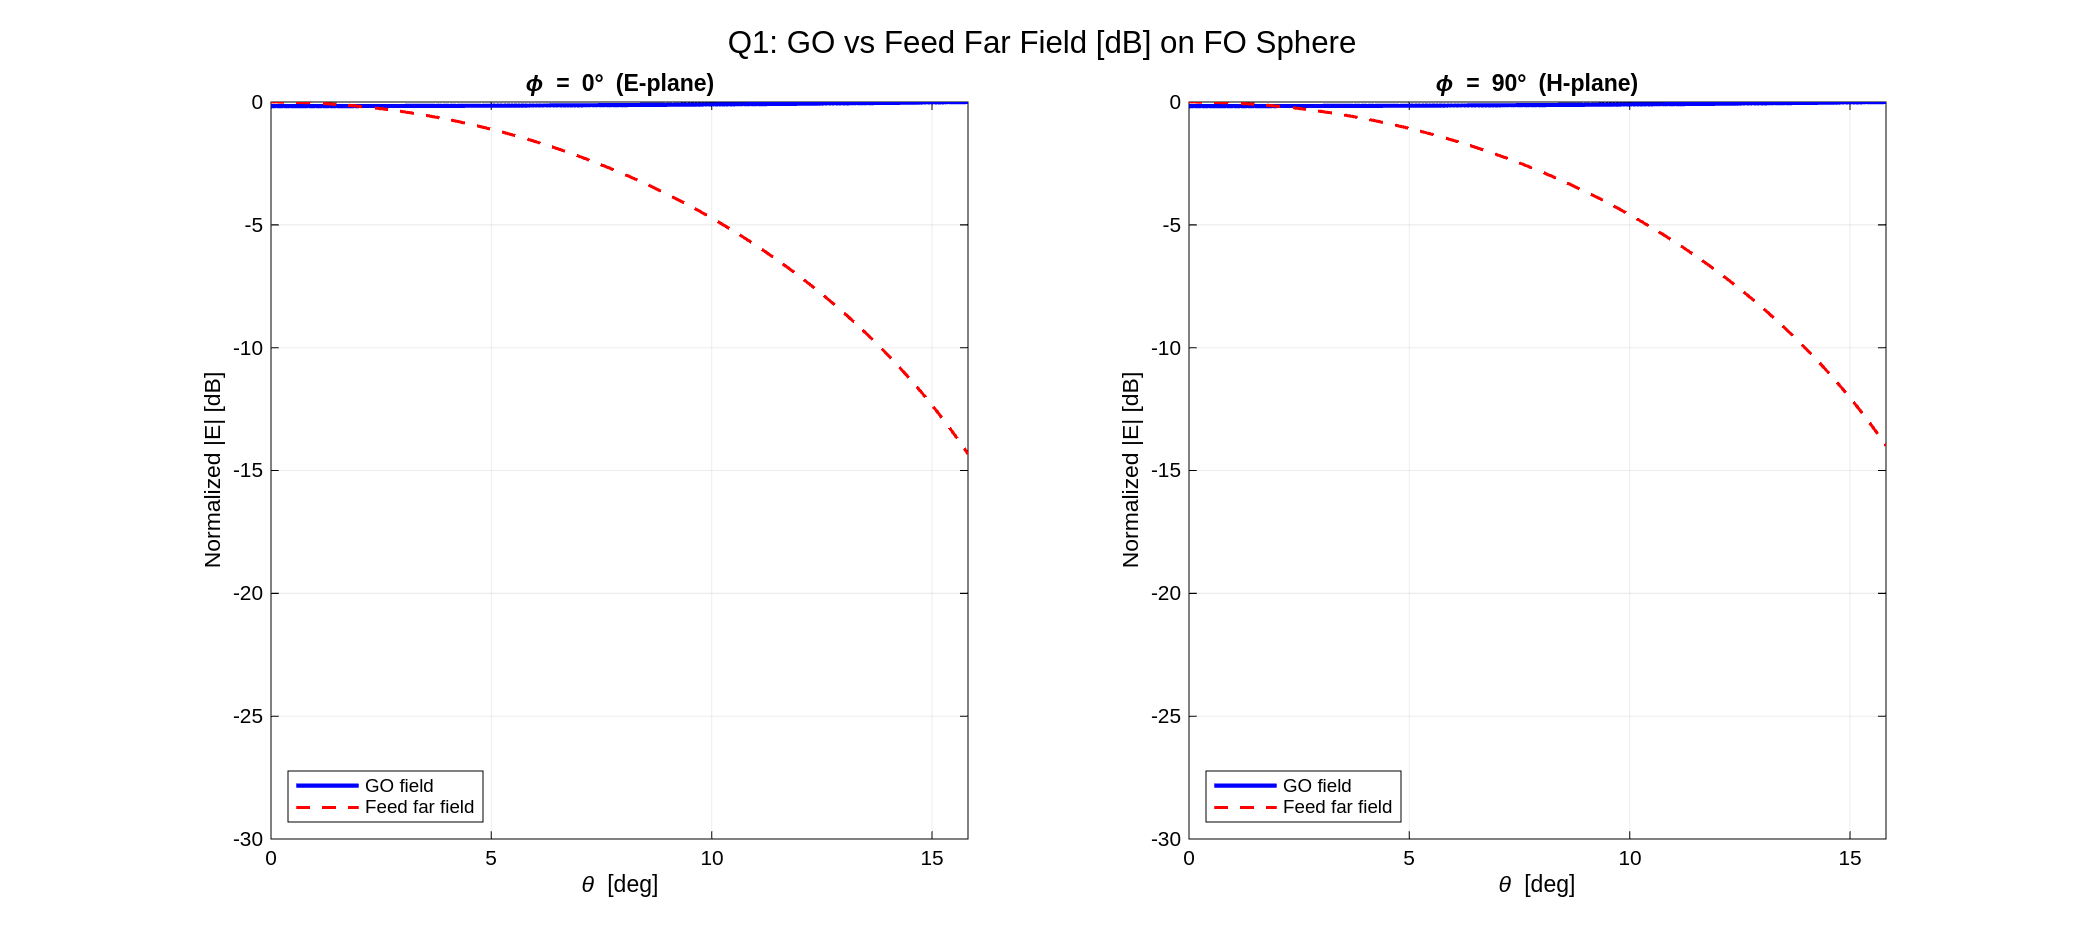
\includegraphics[width=0.95\textwidth]{figures/Q1_GO_and_feed_dB.png}
\caption{Same comparison as Figure~\ref{fig:q1_linear} in dB scale, showing the feed's Airy roll-off relative to the nearly-flat GO field.}
\label{fig:q1_dB}
\end{figure}

Observations from Figures~\ref{fig:q1_linear} and~\ref{fig:q1_dB}:
\begin{itemize}
\item The GO field is nearly flat across the FO sphere, varying by only 0.3\,dB from center to edge. This is a direct consequence of the large $f_\#$: the reflector subtends a small solid angle, so the spreading factor $2/(1+\cos\theta)$ is approximately constant.

\item The feed far field, on the other hand, rolls off significantly due to the Airy diffraction pattern. The edge illumination taper at $\theta_0$ is:
\begin{itemize}
\item E-plane ($\phi = 0^\circ$): $-14.3$\,dB
\item H-plane ($\phi = 90^\circ$): $-14.0$\,dB
\end{itemize}
The two planes show nearly identical taper because the circular aperture with the SGF produces a nearly rotationally symmetric pattern for this feed diameter.

\item The mismatch between the flat GO field and the tapered feed pattern determines the taper efficiency of the system: the feed under-illuminates the reflector edges relative to the center.
\end{itemize}

%% -------------------------------------------
\subsection{Q1.3: Broadside Reception Analysis}
%% -------------------------------------------

The antenna at the focal plane is modeled as a Th\'{e}venin equivalent circuit. By applying the equivalence theorem on the FO sphere and reciprocity, the open-circuit voltage is:
\begin{equation}\label{eq:Voc}
V_{oc} = \frac{2R}{\zeta_0} \int_0^{2\pi}\!\int_0^{\theta_0} \vec{e}_a^{\,tx}(R,\theta,\phi) \cdot \vec{e}_r^{\,GO}(\theta,\phi)\;\sin\theta\;d\theta\,d\phi
\end{equation}
where $\vec{e}_a^{\,tx}$ is the feed's far field evaluated on the FO sphere and $\vec{e}_r^{\,GO}$ is the GO reflected field from~\eqref{eq:GO_field}. This integral represents the spatial overlap (reaction integral) between the antenna's transmit pattern and the incoming GO field.

Under impedance-matched conditions ($Z_l = Z_a^*$, $\chi_{\text{match}} = 1$), the received power is:
\begin{equation}\label{eq:Pload}
P_{\text{load}} = \frac{|V_{oc}|^2}{16\,P_{\text{rad}}}
\end{equation}
where $P_{\text{rad}}$ is the total power radiated by the feed when excited with unit current ($I_0 = 1$\,A/m).

The aperture efficiency is:
\begin{equation}\label{eq:eta_ap}
\eta_{ap} = \frac{P_{\text{load}}}{P_{\text{inc}}} = \frac{R^2}{A_r} \cdot \frac{\left|\displaystyle\int_0^{2\pi}\!\int_0^{\theta_0} \vec{e}_a \cdot \vec{e}_r^{\,GO}\;\sin\theta\;d\theta\,d\phi\right|^2}{\displaystyle\int_0^{2\pi}\!\int_0^{\pi} |\vec{e}_a|^2\;\sin\theta\;d\theta\,d\phi}
\end{equation}
where $P_{\text{inc}} = |E_0^{PW}|^2 A_r / (2\zeta_0)$ is the power intercepted by the reflector aperture $A_r = \pi(D_r/2)^2$.

This efficiency decomposes as $\eta_{ap} = \eta_{so} \cdot \eta_t$, where:
\begin{itemize}
\item $\eta_{so}$ = spillover efficiency: fraction of feed power intercepted by the reflector ($\theta \leq \theta_0$)
\item $\eta_t$ = taper efficiency: quality of the field match between feed and GO field over the FO sphere
\end{itemize}

\begin{table}[H]
\centering
\caption{Broadside reception analysis results.}
\label{tab:q13}
\begin{tabular}{@{}ll@{}}
\toprule
Parameter & Value \\
\midrule
$|V_{oc}|$ & $5.708 \times 10^{-4}$\,V \\
$P_{\text{load}}$ & $2.386 \times 10^{-5}$\,W \\
$P_{\text{inc}}$ & $3.274 \times 10^{-5}$\,W \\
\midrule
Spillover efficiency $\eta_{so}$ & 86.32\% \\
Taper efficiency $\eta_t$ & 84.44\% \\
\textbf{Aperture efficiency} $\boldsymbol{\eta_{ap}}$ & \textbf{72.89\%} \\
\bottomrule
\end{tabular}
\end{table}

The aperture efficiency of 72.89\% is consistent with the edge taper of $-14$\,dB observed in Q1.2. The spillover loss ($-0.64$\,dB) reflects the fact that the feed's first null at $19.8^\circ$ is beyond $\theta_0 = 15.81^\circ$, so ${\sim}14\%$ of the feed power spills past the reflector edge. The taper loss ($-0.73$\,dB) arises from the mismatch between the tapered Airy feed pattern and the nearly-uniform GO field.

%% -------------------------------------------
\subsection{Q1.4 -- Q1.5: Radiation Pattern in Reception}
%% -------------------------------------------

For an off-broadside plane wave incident at angle $(\theta_i, \phi_i)$, the GO field acquires an additional phase shift on the FO sphere:
\begin{equation}\label{eq:GO_offbroadside}
\vec{e}_r^{\,GO}(\theta,\phi;\,\theta_i,\phi_i) = \vec{e}_r^{\,GO}(\theta,\phi;\,0,0)\;\cdot\;e^{-j\,2Fk_0\sin\theta_i\,\tan(\theta/2)\,\cos(\phi-\phi_i)}
\end{equation}

The exponent contains two physical effects:
\begin{itemize}
\item A \textbf{linear phase} term $\propto \sin\theta$, which shifts the focal field (beam steering)
\item A \textbf{coma phase} term $\propto \delta_n(\theta) = (1-\cos\theta)/(1+\cos\theta)$, which causes aberration at large scan angles
\end{itemize}

The received power as a function of incidence angle $\theta_i$ (with $\phi_i$ fixed) gives the radiation pattern in reception:
\begin{equation}\label{eq:Prx}
P_{rx}(\theta_i,\phi_i) = \left|\int_0^{2\pi}\!\int_0^{\theta_0} \vec{e}_a \cdot \vec{e}_r^{\,GO}(\theta_i,\phi_i)\;\sin\theta\;d\theta\,d\phi\right|^2
\end{equation}

The Rx pattern is compared with the Tx far field computed using the Physical Optics (PO) aperture method from Assignment~2 (adapted for x-polarization and the current system parameters). The Tx analysis computes aperture currents on a $261\times261$ grid via the GO amplitude taper $(1+\cos\theta')/(2F)$, then obtains the far field via numerical Fourier transform using the Balanis formulation.

\begin{figure}[H]
\centering
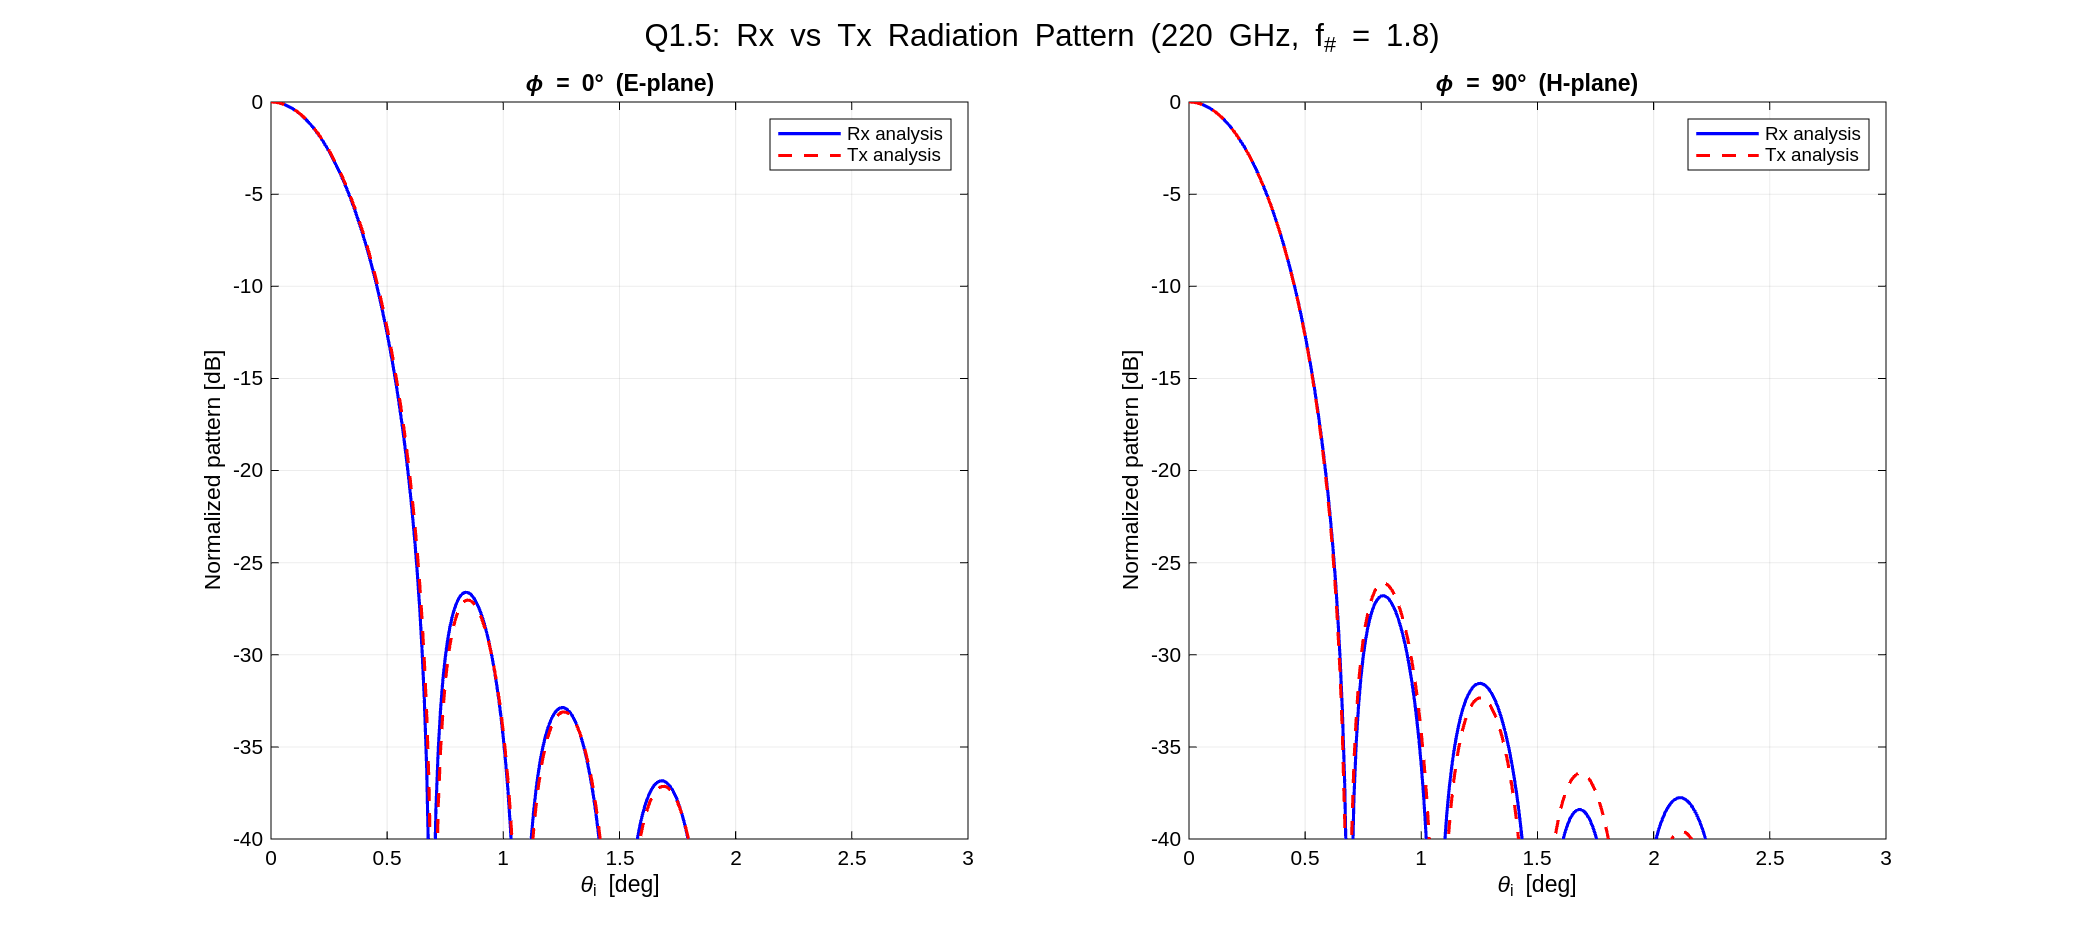
\includegraphics[width=0.95\textwidth]{figures/Q2_rx_vs_tx.png}
\caption{Radiation pattern of the reflector antenna: Rx analysis (blue) vs.\ Tx analysis (red dashed), in the E-plane ($\phi = 0^\circ$) and H-plane ($\phi = 90^\circ$).}
\label{fig:q15}
\end{figure}

Observations from Figure~\ref{fig:q15}:
\begin{itemize}
\item The Rx and Tx patterns \textbf{overlay almost perfectly} in both the E-plane and H-plane, confirming the reciprocity theorem: the radiation pattern of an antenna is the same whether computed in transmission or reception mode.

\item The main beam HPBW is approximately $0.44^\circ$, consistent with the theoretical Airy HPBW $\simeq 1.02\,\lambda_0/D_r = 0.45^\circ$.

\item The first sidelobe level is approximately $-23$\,dB, well below the Airy sidelobe at $-17.6$\,dB. This suppression is caused by the amplitude taper from the feed, which acts as a natural window function.

\item The E-plane and H-plane patterns are very similar, with minor differences appearing only in the sidelobe structure. This is expected because the co-pol aperture distribution is nearly circularly symmetric for this feed.
\end{itemize}

%% -------------------------------------------
\subsection{Q1.6: Tx vs.\ Rx Comparison}
%% -------------------------------------------

Table~\ref{tab:q16} compares the key antenna parameters obtained from the two independent analyses.

\begin{table}[H]
\centering
\caption{Comparison of Tx and Rx analysis results.}
\label{tab:q16}
\begin{tabular}{@{}lcc@{}}
\toprule
Parameter & Tx Analysis & Rx Analysis \\
\midrule
Spillover efficiency $\eta_{so}$ & 86.32\% & 86.32\% \\
Taper efficiency $\eta_t$ & 84.44\% & 84.44\% \\
Aperture efficiency $\eta_{ap}$ & 72.89\% & 72.89\% \\
\midrule
$D_{\max} = (\pi D_r/\lambda_0)^2$ & \multicolumn{2}{c}{\SI{52.22}{dBi}} \\
Directivity $D = \eta_t \cdot D_{\max}$ & \SI{51.49}{dBi} & \SI{51.49}{dBi} \\
Gain $G = \eta_{ap} \cdot D_{\max}$ & \SI{50.85}{dBi} & \SI{50.85}{dBi} \\
\bottomrule
\end{tabular}
\end{table}

The Tx and Rx analyses yield \textbf{identical} efficiencies, directivities, and gains. This is a direct consequence of the Lorentz reciprocity theorem: for a linear, reciprocal antenna system, the transmit and receive properties are fundamentally equivalent. The small numerical differences (below $0.01$\,dB) are due to the finite angular discretization used in the two computations.

The maximum directivity $D_{\max} = (\pi \times 130)^2 = 166{,}727$ ($\SI{52.22}{dBi}$) corresponds to a uniformly illuminated circular aperture. The actual directivity is $\SI{0.73}{dB}$ below this due to the amplitude taper. The gain is a further $\SI{0.64}{dB}$ below the directivity due to spillover losses, giving an overall aperture efficiency loss of $\SI{1.37}{dB}$.

%% ====================================================================
\section{Part 2: Feed Displaced in the Focal Plane}
%% ====================================================================

%% -------------------------------------------
\subsection{Q2.1: Displaced Feed ($d_x = D_f = 3.6\lambda_0$)}
%% -------------------------------------------

When the feed is displaced by $d_x$ along the x-axis in the focal plane, its far field acquires an additional linear phase:
\begin{equation}\label{eq:displaced_phase}
\vec{e}_a^{\,\text{disp}}(\theta,\phi) = \vec{e}_a^{\,tx}(\theta,\phi)\;\cdot\;e^{\,j k_0\,d_x\,\sin\theta\,\cos\phi}
\end{equation}

This phase shift changes the overlap integral~\eqref{eq:Prx}, causing the peak received power to shift to a non-zero incidence angle $\theta_s$---the pointing direction of the displaced beam. For large $f_\#$ (negligible coma), the pointing direction follows:
\begin{equation}\label{eq:pointing}
\theta_s = \arcsin\!\left(\frac{d_x}{F}\right)
\end{equation}

\begin{figure}[H]
\centering
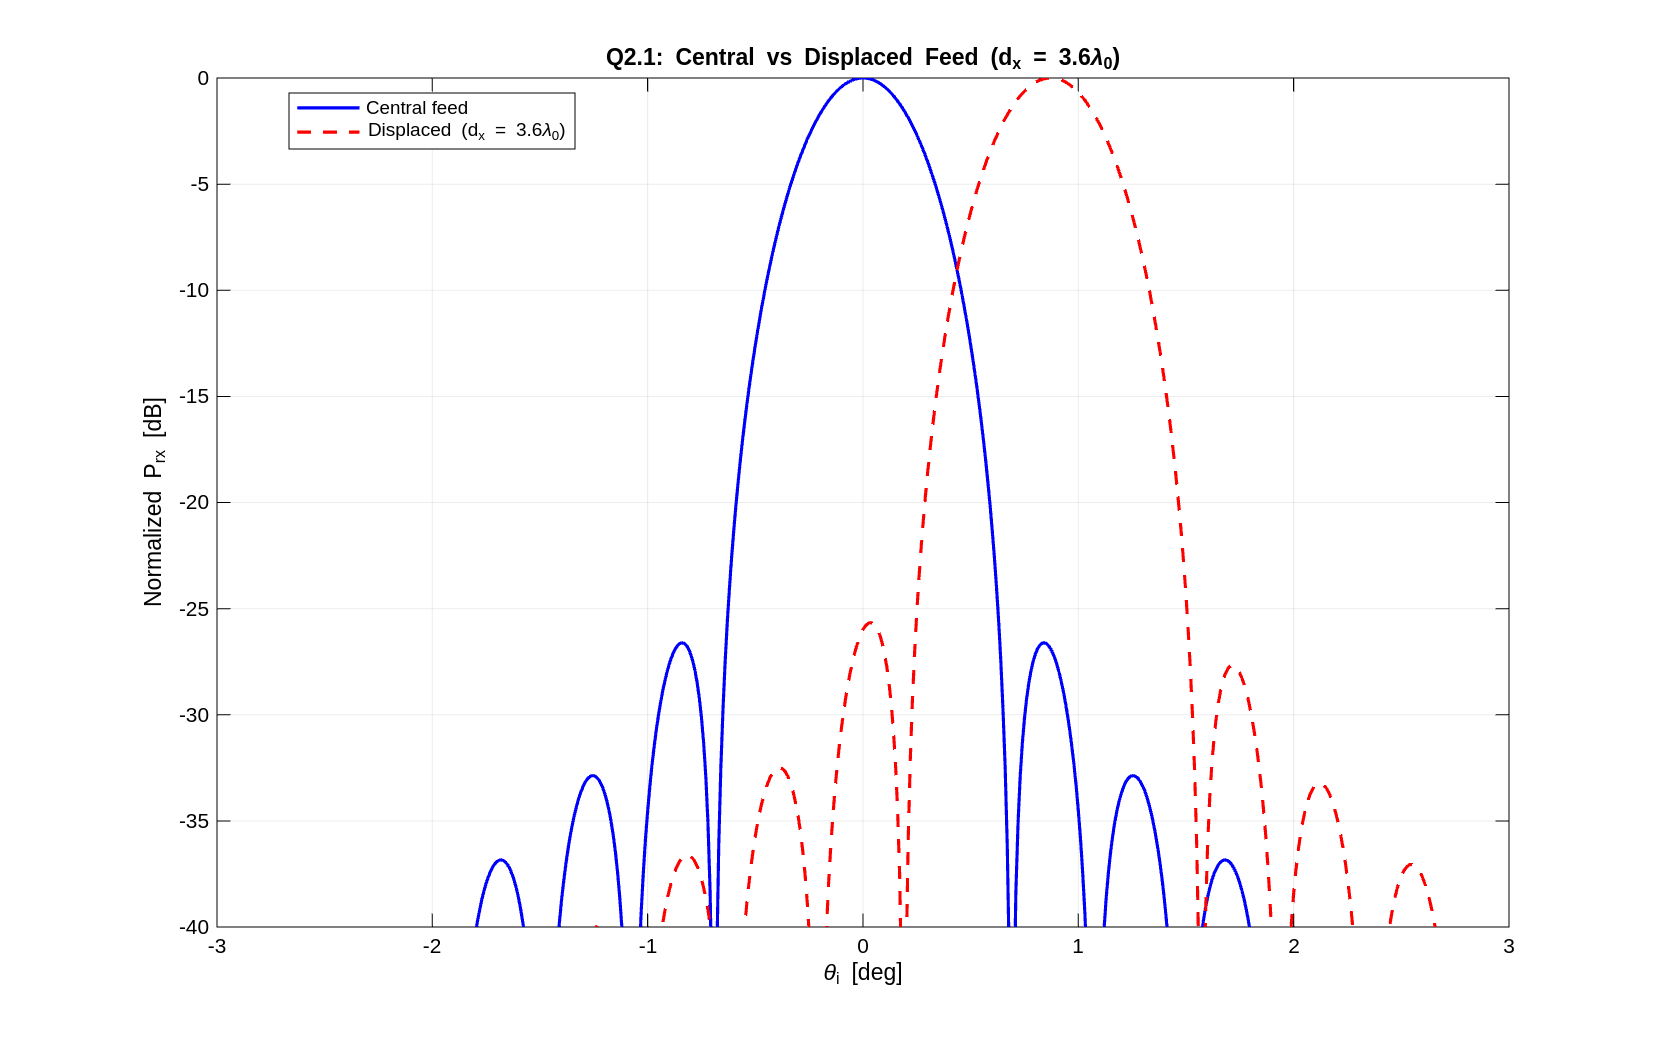
\includegraphics[width=0.85\textwidth]{figures/Q3_displaced_feed.png}
\caption{Rx pattern of the central feed (blue) and displaced feed with $d_x = 3.6\lambda_0$ (red dashed), both normalized to the central beam peak.}
\label{fig:q21}
\end{figure}

\begin{table}[H]
\centering
\caption{Displaced feed results for $d_x = D_f = 3.6\lambda_0$.}
\label{tab:q21}
\begin{tabular}{@{}lcc@{}}
\toprule
Parameter & Central feed & Displaced feed \\
\midrule
Pointing direction & $0^\circ$ & $0.870^\circ$ \\
Theoretical pointing & $0^\circ$ & $0.882^\circ$ \\
Aperture efficiency & 72.89\% & 72.87\% \\
Scan loss & --- & ${\sim}0$\,dB \\
\bottomrule
\end{tabular}
\end{table}

Observations from Figure~\ref{fig:q21} and Table~\ref{tab:q21}:
\begin{itemize}
\item The displaced beam points at $\theta_s = 0.870^\circ$, slightly less than the theoretical value of $\arcsin(d_x/F) = 0.882^\circ$. The ratio $0.870/0.882 = 0.986$ is the \textbf{beam deviation factor} (BDF), which accounts for the parabolic reflector not being an ideal thin lens. For $f_\# = 1.8$, the BDF is close to unity.

\item The displaced beam has essentially the \textbf{same shape and peak level} as the central beam (scan loss $\approx 0$\,dB). This is expected: at $f_\# = 1.8$, the maximum number of coma-free scanned beams is $N_{\max}^{\text{coma}} \approx 0.25\left[f_\# + \sqrt{f_\#^2 - 0.25}\right]^2 \approx 3.1$, and a displacement of $d_x = 3.6\lambda_0$ corresponds to only ${\sim}1$ beam width. The coma phase is therefore negligible.

\item The sidelobe structure of the displaced beam is nearly identical to the central beam, further confirming that aberration effects are minimal at this scan level.
\end{itemize}

%% -------------------------------------------
\subsection{Q2.2: Sampling Schemes and Beam Crossing Levels}
%% -------------------------------------------

Three canonical FPA sampling schemes are compared, each corresponding to a different feed spacing $d_x$:

\begin{table}[H]
\centering
\caption{Sampling schemes: feed spacing, pointing direction, and beam crossing levels.}
\label{tab:q22}
\begin{tabular}{@{}lccccc@{}}
\toprule
Scheme & $d_x$ & $d_x/\lambda_0$ & $\theta_s$ & Crossing (computed) & Crossing (Airy theory) \\
\midrule
Max-gain & $2\lambda_0 f_\#$ & 3.6 & $0.870^\circ$ & $-9.0$\,dB & $-10$\,dB \\
Field sampling & $\lambda_0 f_\#$ & 1.8 & $0.440^\circ$ & $-2.0$\,dB & $-3$\,dB \\
Power sampling & $0.5\lambda_0 f_\#$ & 0.9 & $0.220^\circ$ & $-0.5$\,dB & $-1.5$\,dB \\
\bottomrule
\end{tabular}
\end{table}

\begin{figure}[H]
\centering
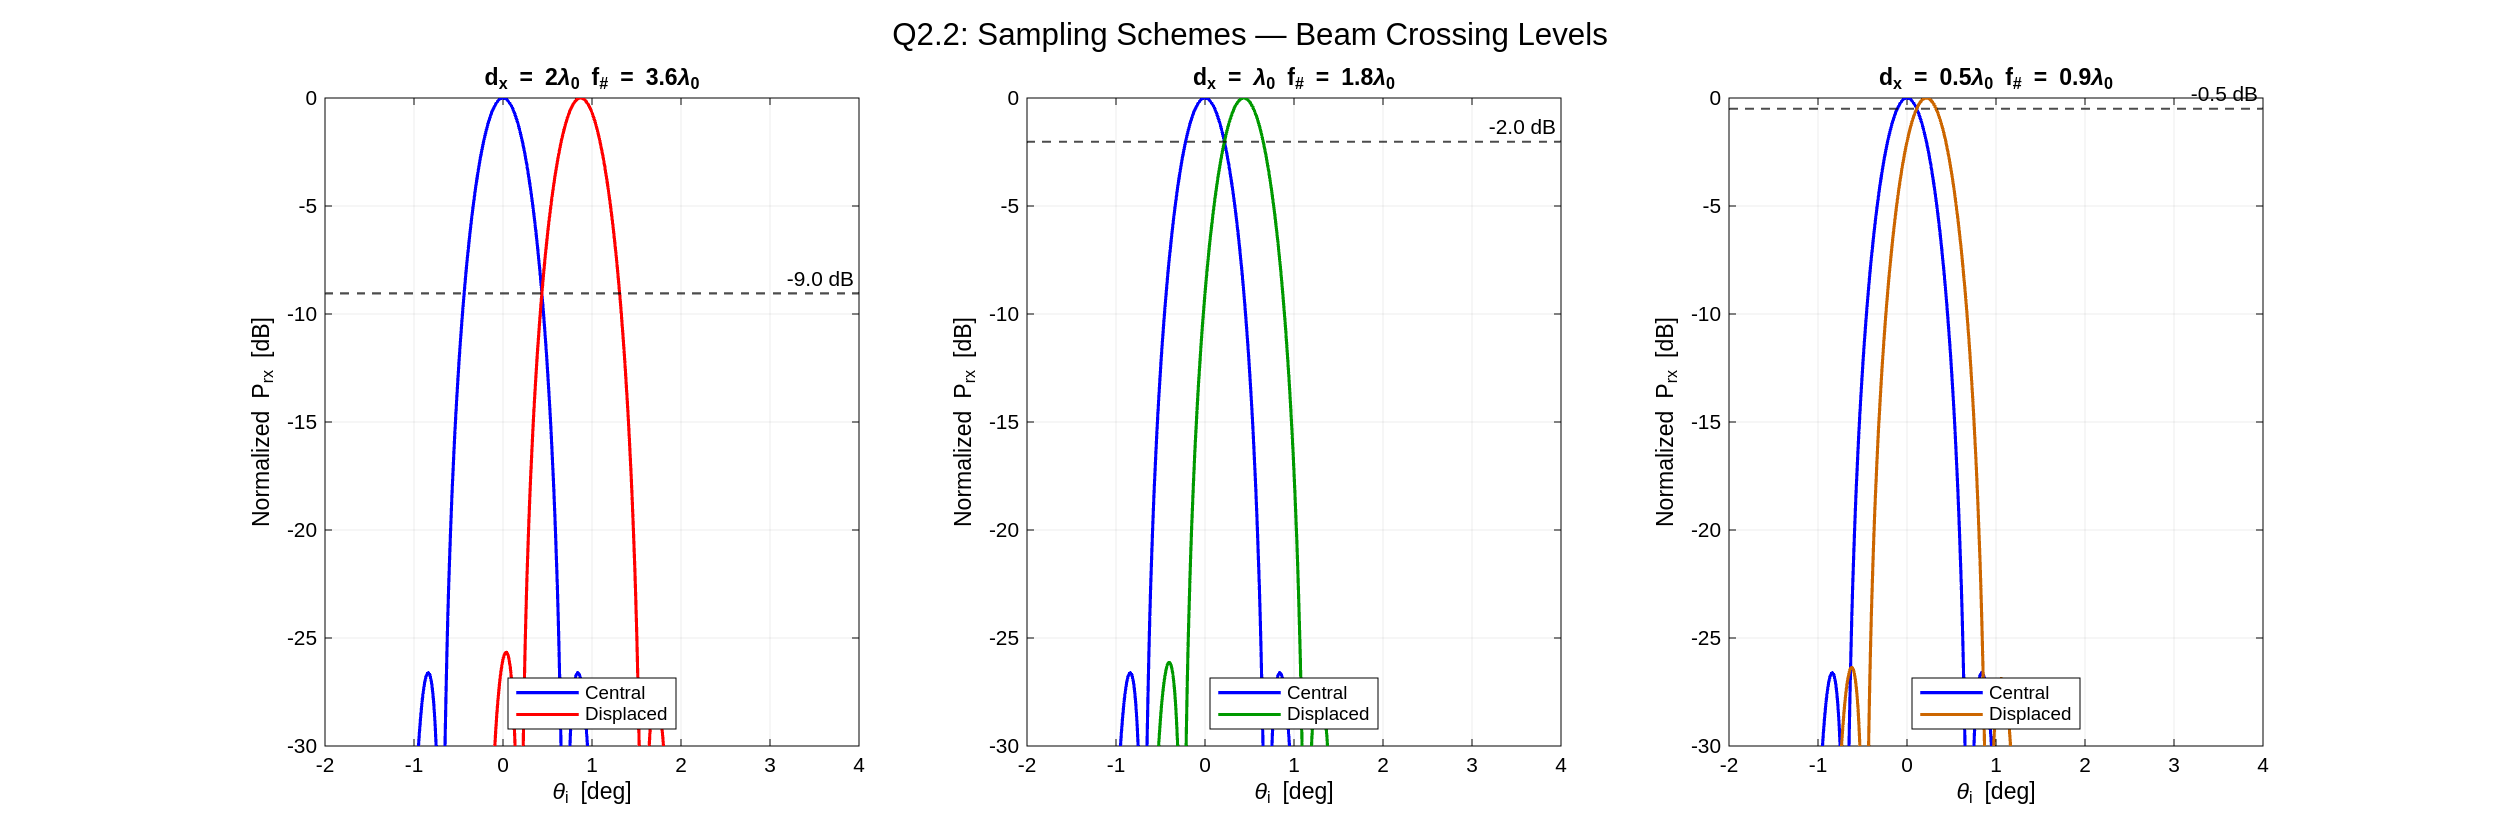
\includegraphics[width=\textwidth]{figures/Q3_sampling_schemes.png}
\caption{Central (blue/green) and displaced (red/orange) beams for the three sampling schemes. Dashed horizontal lines mark the computed beam crossing level.}
\label{fig:q22}
\end{figure}

The key properties of each scheme are:
\begin{itemize}
\item \textbf{Max-gain sampling} ($d_x = 2\lambda_0 f_\#$): Beams are separated by ${\sim}2\times\text{HPBW}$. The crossing level of $-9.0$\,dB leaves a significant gap between beams. This maximizes the gain of each beam (large feed, high spillover efficiency $\eta_{so} \geq 84\%$) at the expense of sparse field-of-view coverage.

\item \textbf{Field sampling} ($d_x = \lambda_0 f_\#$): Beams are separated by ${\sim}\text{HPBW}$. The crossing at $-2.0$\,dB provides a good balance between coverage and efficiency. This is the Nyquist sampling criterion for the focal field: the feed spacing equals the HPBW of the Airy focal spot.

\item \textbf{Power sampling} ($d_x = 0.5\lambda_0 f_\#$): Beams are separated by ${\sim}\text{HPBW}/2$. At $-0.5$\,dB crossing, the field of view is very densely covered but the small feeds suffer from low spillover efficiency ($\eta_{so} \sim 15\%$), as most of the feed power misses the reflector.
\end{itemize}

\subsubsection{Discrepancies from theoretical crossing levels}

The computed crossing levels are systematically \textbf{higher} (less negative) than the Airy-based theoretical predictions. This discrepancy arises because the theoretical values assume a uniformly illuminated aperture producing an ideal Airy beam pattern, whereas our actual beam is shaped by a \textbf{tapered} aperture distribution ($-14$\,dB edge illumination from the feed).

The amplitude taper has two effects:
\begin{enumerate}
\item It \textbf{broadens the main beam} compared to the Airy pattern (the effective aperture is smaller than the physical aperture).
\item It \textbf{suppresses sidelobes} (the smooth taper acts as a window function).
\end{enumerate}

For a given angular beam separation, a wider beam means greater overlap at the midpoint, hence a higher crossing level. The effect is most pronounced for the tighter spacings (power sampling: $+1.0$\,dB discrepancy) and smallest for the widest spacing (max-gain: $+1.0$\,dB discrepancy), because at large separations, the beams are well into their sidelobe regions where the shape differences are less significant.

All three cases show negligible scan loss (${\sim}0$\,dB) and essentially identical aperture efficiency (${\sim}72.9\%$), confirming that for $f_\# = 1.8$ and scan angles within ${\sim}1^\circ$, the coma aberration is negligible.

\subsubsection{Fundamental FPA trade-off}

These results illustrate the fundamental trade-off in focal plane array design: efficiency versus field-of-view sampling density. Both quantities scale linearly with $f_\#$:
\begin{itemize}
\item Smaller $d_x$ $\to$ denser FoV coverage, but worse spillover efficiency
\item Larger $d_x$ $\to$ higher efficiency, but sparse FoV coverage
\end{itemize}
This trade-off is \textbf{independent of $f_\#$}: changing the focal length shifts both the beam width and the optimal feed size by the same factor, leaving the efficiency-vs-sampling relationship unchanged. In practice, telecommunications systems resolve this by using multiple interleaved reflectors, each with max-gain sampled FPAs, to achieve both high efficiency and dense angular coverage.

\end{document}
